\section{Des contraintes architecturales}

\paragraph{} Cependant, le choix de l'architecture que l'on souhaite mettre en place de manière \emph{globale} doit 
être sagement réfléchi. En effet, les contraintes d'un tel déploiement et de l'ampleur de l'utilisation de ce système
doivent être clairement identifiées et adressées dans le choix même de l'architecture.

\paragraph{} Le premier obstacle à une mise en place d'un service à grande échelle est la \emph{scalabilité}, c'est-à-dire
la capacité qu'a un service à s'adapter à un plus grand trafic tout en conservant une qualité de service et des performances
identiques ; en bref, c'est sa capacité à \emph{monter en charge} \cite{Scalability0}. Il s'agit là d'un enjeu critique pour
un service dont l'ambition est d'être déployé et utilisé à l'échelle mondiale ; elle devra donc être capable de prendre en
charge une forte montée du trafic à un instant \emph{T} sans que l'expérience utilisateur n'en soit pour autant affectée.

\paragraph{} La \emph{résilience}, c'est-à-dire la \emph{tolérance à la panne}, est le second obstacle qui devra être franchi.
En effet, aussi performante soit-elle, une application ne sera jamais capable de durer dans le temps si elle subit ne serait-ce
que de courtes périodes d'inaccessibilité de manière répétée. Ainsi, un service résilient est en capacité de fournir une
\emph{continuité de service} quand bien même certains de ses composants viendraient à cesser de fonctionner.

\paragraph{} Mais dans un système fortement distribué, la \emph{latence} est le prix à payer de la résilience. Cette dernière nécessiterait
la mise en disponibilité du service dans de nombreuses zones géographiques, réduisant par là même les risques de sinistre. Il serait alors
nécessaire, soit de mettre en place un cache applicatif ou un CDN (\emph{Content Delivery Network}) pour optimiser les 
accès aux ressources ; des serveurs proxy ou des tunnels dédiés pour accéder directement au service ; voire de déployer plusieurs
instances de l'application dans les différentes régions couvertes, ce qui nécessiterait une gestion adéquat des \emph{états}
au sein de l'application ainsi que de prévoir un moyen de resynchroniser l'ensemble des données si cela s'avérait nécessaire.

\paragraph{} Il est important d'avoir conscience que la réponse apportée à un problème d'architecture peut elle-même révéler 
d'autres questions \& challenges.

\paragraph{} Pour étudier les solutions que l'on peut apporter à ces différentes contraintes, nous vous proposons d'étudier
ci-dessous trois architectures qui adressent chacune d'entre elles de manière différente, disposant de leurs propres
avantages et inconvénients.


\paragraph{Architecture Monolithique}

\paragraph{} Parler de \emph{monolithe} est de nos jours presque une insulte dans le monde du développement logiciel. Nous 
l'utilisons - à l'instar du \emph{legacy} - comme un terme péjoratif, sous-entendant que le projet est dôté d'une \emph{codebase}
mal architecturée, aux couplages forts et aux déploiements longs et laborieux.

\paragraph{} Mais saviez-vous que \url{https://StackExchange.com}, ainsi que ses \emph{plus de 170 sites} de questions-réponses
communautaires (dont \url{https://StackOverflow.com}, bien connu des développeurs) étaient des applications monolithiques 
parvenant à maintenir un temps de réponse moyen de \emph{11.80 millisecondes} \cite{Microservices7} ?

\begin{figure}[h]
    \centering
    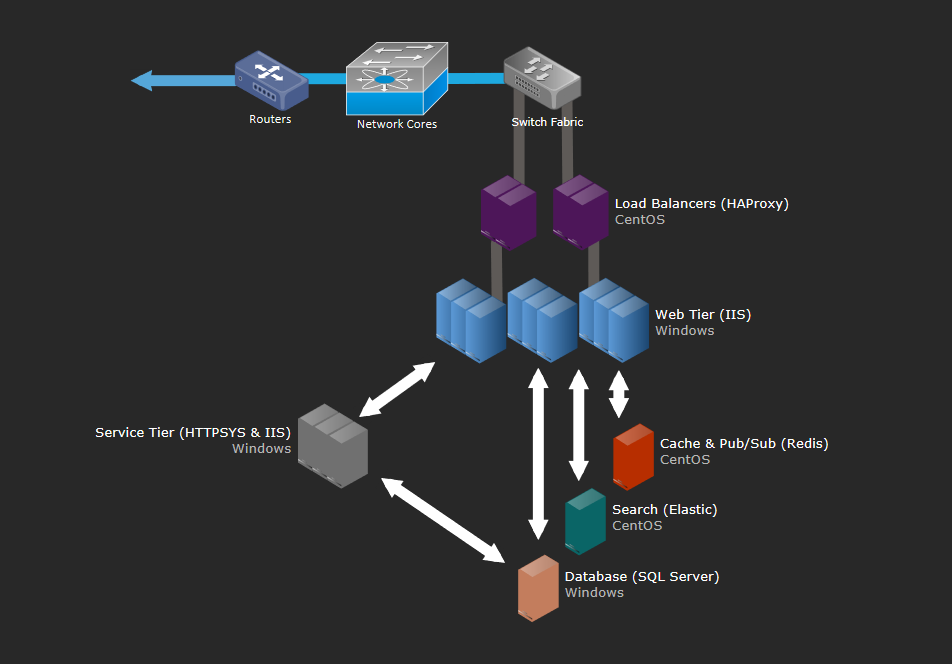
\includegraphics[width=400px]{chapters/02/images/stackexchange.png}
    \caption{\label{stackexchange_architecture} Architecture des services StackExchange.}
\end{figure}

\paragraph{} Il est donc important de savoir raison garder. Tout d'abord, le grand avantage d'une architecture monolithique
est que le développement et le déploiement de l'application sont en théorie plus simples à effectuer. La maintenance et 
les évolutions applicatives dépendent quant à elles fortement du couplage des composants au sein même de l'application et 
de la qualité générale de la \emph{codebase}. De même, la latence est normalement assez faible au sein de la solution car,
hors systèmes externes, les appels ne consistent qu'à des exécutions en mémoire.

\paragraph{} Cependant, le monolithe pouvant être amené à grossir rapidement, il va lier très fortement l'équipe de développement
à une \emph{stack technologique} qu'il sera potentiellement laborieux de faire évoluer. Les changements de version peuvent 
nécessité une quantité non négligeable de développement s'ils ne sont pas rétro-compatibles, sans parler d'un changement 
complet de technologie alors que le projet a déjà plusieurs années de vie derrière lui.

\paragraph{} Enfin, la scalabilité peut s'avérer être une contrainte complexe à abattre, d'autant plus si le monolithe
conserve un \emph{état}, quel qu'il soit, durant son \emph{runtime}. Ainsi, il est bien souvent nécessaire de mettre en place
des solutions supplémentaires pour servir de pont entre les utilisateurs et le service : on parle alors de \emph{2\up{nd} layer},
ou \emph{seconde couche}, qui sera alors responsable de la répartition de la charge entre les différentes instances de l'application
(comme illustré sur la figure \ref{stackexchange_architecture}). Si un état est conservé, un \emph{store} pourra être commun
à l'ensemble des instances pour qu'elles puissent le récupérer et le mettre à jour si nécessaire.


\paragraph{Microservices}

\paragraph{} Gagnant en popularité depuis les quatre dernières années, l'architecture microservices part d'un postulat
simple : s'il devient compliqué de faire évoluer une application monolithique et de conserver un couplage faible entre ses
composants, il suffit de l'éclater en multiples \emph{microservices} intéragissant entre eux et prenant chacun en charge 
un aspect de la logique métier de l'application.

\begin{figure}[h]
    \centering
    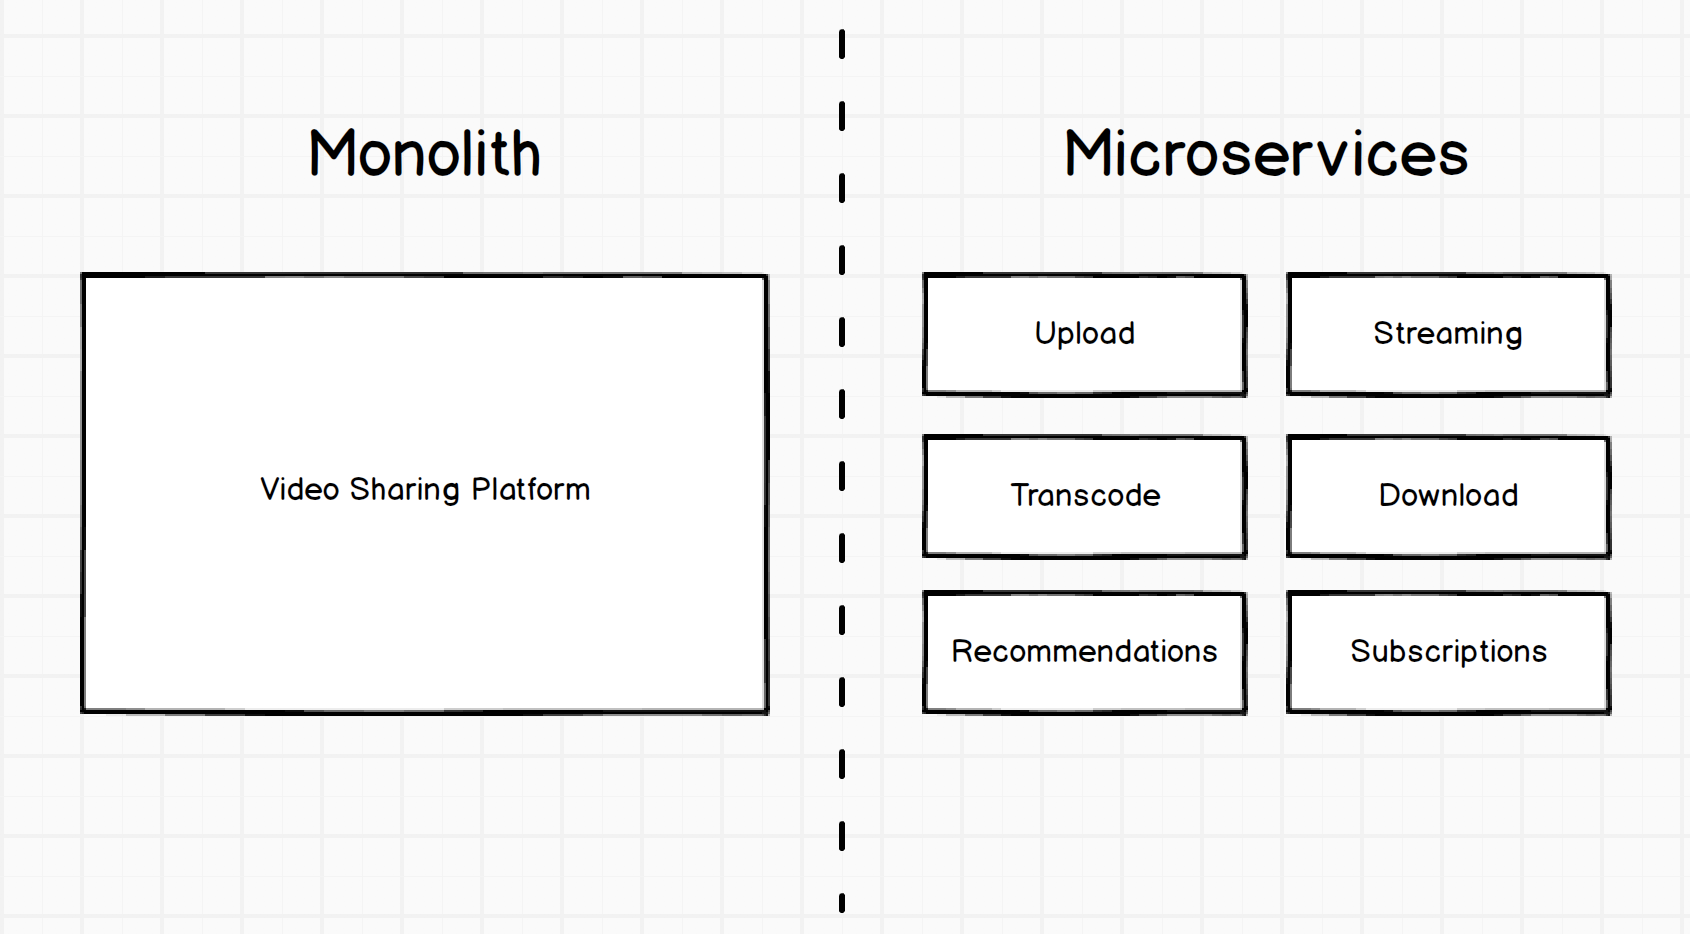
\includegraphics[width=350px]{chapters/02/images/monolith_to_microservices.png}
    \caption{\label{monolith_to_microservices} Exemple de transformation en microservices d'une plateforme de partage vidéo. \cite{Microservices1}}
\end{figure}

\paragraph{} Les avantages d'une telle architecture sont multiples :

\paragraph{} Tout d'abord, cela permet une meilleure scalabilité du système dans son ensemble. Dans l'exemple de la plateforme
de partage de vidéo de la figure \ref{monolith_to_microservices}, s'il y a beaucoup plus de visionnages que de mises en 
ligne sur le service, il sera alors possible d'allouer plus de ressources au service \emph{Streaming} ou d'en déployer
plusieurs instances \emph{sans impacter les autres services}. Les économies en terme de ressources sont énormes car, dans 
le cas d'une architecture monolithique, une augmentation des ressources n'aurait qu'en partie bénéficié à la fonctionnalité 
concernée, et le déploiement d'une nouvelle instance concernerait évidemment l'application toute entière.

\paragraph{} Il est possible de réutiliser certains composants si le couplage entre ces derniers est \emph{faible}.
Ainsi, si plusieurs projets au sein d'une entreprise disposent de certaines fonctionnalités en commun, il leur est possible 
de réutiliser un microservice déjà déployé en production pour satisfaire leur besoin. C'est ici que l'importance d'un couplage
faible se fait réellement ressentir : si l'intégralité des services dépendent les uns des autres, il est impossible de les
réutiliser séparément en dehors du contexte de leur projet d'origine.

\paragraph{} De plus, chaque service peut aussi être déployé indépendament des autres. Cela permet une plus grande flexibilité dans
les cycles de développement de nouvelles fonctionnalités, augmentant la vélocité de l'équipe tout en réduisant les risques.
Une mise à jour dans le composant \emph{Recommendations}, même si elle induisait une indisponibilité totale de cette fonctionnalité,
serait quasiment invisible pour les utilisateurs qui continueraient d'utiliser le reste du service.

\paragraph{} Enfin, cette architecture permet une forte résilience du système, qui peut alors rester - partiellement - 
opérationel quand bien même l'un de ses composants viendrait à cesser de fonctionner. Ainsi, si le composant \emph{Upload}
devenait innacessible, seule la mise en ligne de vidéos deviendrait inaccessible ; l'intégralité des utilisateurs aurait
toujours la possibilité de visionner les vidéos présentes sur la plateforme.

\paragraph{} Oui, mais.

\paragraph{} Si, pris indépendament, le déploiement d'\emph{un} service est simplifié, il est important de conserver
à l'esprit l'\emph{ensemble} de l'architecture dont le déploiement est, lui, énormément complexifié. Là où il suffisait de 
déployer un service lors d'une mise à jour impactant l'ensemble des fonctionnalités, il est désormais nécessaire de procéder 
à de nombreux déploiement simultanés, voire parfois séquentiels !

\paragraph{} De même, la gestion de l'ensemble de ces microservices requiert un brin d'infrastructure supplémentaire.
Un registre permettant d'effectuer du \emph{service discovery} est nécessaire pour savoir où se situe un service particulier.
Un \emph{circuit breaker} est nécessaire pour permettre un \emph{mode dégradé} du système au cas où un service viendrait
à s'effondrer. Un \emph{serveur de configuration} est judicieux pour centraliser la configuration de l'ensemble des services
composant la nouvelle infrastructure. Un \emph{proxy} et un \emph{load balancer} pour abstraire la complexité de l'infrastructure
aux consommateurs du service et répartir la charge entre les différentes instances. Si l'aspect métier bénéficie grandement
de cette architecture, l'infrastructure n'en est que plus complexe à gérer.

\paragraph{} Enfin, la latence \emph{peut} devenir un problème de taille si l'architecture n'a pas été correctement conçue.
Ainsi, concevoir chaque microservice comme une API REST communiquant entre elles grâce à des appels HTTP synchrones est à
\emph{proscrire absolument}. Il est alors nécessaire de mettre en place un \emph{bus de message} (\emph{message broker})
permettant la production et la consommation asynchrone de messages (ou \emph{événements}) au sein du système. En fonction
de la tâche qu'il devra accomplir, chaque microservice pourra alors \emph{produire} un message dans le message broker qui
sera \emph{consommé} par un ou plusieurs autres microservices qui se seront au préalable \emph{abonnés} à ce type de messages.
Cela permet de créer un système totalement asynchrone, ne réagissant qu'à des \emph{événements} survenant en son sein.


\paragraph{Blockchain} \cite{Blockchain0} \cite{Blockchain1}

\paragraph{TODO} Étude de cas : la blockchain. Distribution des acteurs et des données, grande résilience du réseau mais scalabilité
du système et latence - en fonction de la technologie - potentiellement accompagnée d'un coût d'usage élevé.

\paragraph{TODO} Problèmes de scalabilité à prendre en compte avec les technologies blockchain :

\begin{itemize}
    \item ETH : CryptoKitties (\url{https://www.cryptokitties.co/}) qui a embourbé le réseau en novembre 2017. 
    Développement d'une solution de scaling : le \emph{Sharding}, \url{https://github.com/ethereum/sharding/blob/develop/docs/doc.md}
    \item BTC : augmentation des frais de transaction due à l'intense usage du réseau.
    Soft fork avec SegWit, servant de bases à deux solutions au problème de scalabilité : SegWit2x, hard fork du réseau,
    et Lightning Network, une solution off-chain permettant l'ouverture et la fermeture de canaux transactionnels par dessus
    le réseau Bitcoin.
\end{itemize}


\paragraph{Un Réseau hétérogène}

\paragraph{TODO} L'hétérogénité n'est pas un frein à l'unité. L'unité c'est le tout.
